\documentclass[a4paper]{article}
\usepackage[utf8]{inputenc}
\usepackage[T1]{fontenc}
\usepackage[pdftex]{graphicx}
\usepackage{fancyhdr}
\usepackage{lscape}
\usepackage{color}
\usepackage{qtree}
\usepackage[english]{babel}
\usepackage{graphicx}
\usepackage[colorinlistoftodos]{todonotes}
\usepackage{listings}
\usepackage{color}
\usepackage{float}
\usepackage{changepage}
\usepackage[margin=1in]{geometry}
\definecolor{codegreen}{rgb}{0,0.6,0}
\definecolor{codegray}{rgb}{0.5,0.5,0.5}
\definecolor{codepurple}{rgb}{0.58,0,0.82}
\definecolor{backcolour}{rgb}{0.95,0.95,0.92}
\usepackage[parfill]{parskip}
 \usepackage{ragged2e}
 \lstdefinestyle{mystyle}{
 	backgroundcolor=\color{backcolour},   
 	commentstyle=\color{codegreen},
 	keywordstyle=\color{magenta},
 	numberstyle=\tiny\color{codegray},
 	stringstyle=\color{codepurple},
 	basicstyle=\footnotesize,
 	breakatwhitespace=false,         
 	breaklines=true,                 
 	captionpos=b,                    
 	keepspaces=true,                 
 	numbers=left,                    
 	numbersep=5pt,                  
 	showspaces=false,                
 	showstringspaces=false,
 	showtabs=false,                  
 	tabsize=2
 }
 
\lstset{
	style=mystyle,
	inputencoding=utf8,
	extendedchars=true,
	literate={á}{{\'a}}1 {ã}{{\~a}}1 {é}{{\'e}}1,
	escapechar=\&
}
\title{Algorithmique et structures de données : Mission 5}
\date{21 novembre 2014}
\author{Groupe 1.2: Ivan Ahad - Jérôme Bertaux - Rodolphe Cambier \\ 
	Baptiste Degryse - Wojciech Grynczel - Charles Jaquet}



\begin{document}
\maketitle

\paragraph*{Question 1 (Cambier Rodolphe)}
L'avantage du tas, c'est la possibilité de récupérer l'élément le plus grand de la file de priorité en O(1), tandis que la liste le fera en O(n) où n est le nombre d'éléments de celle-ci.

Cependant, l'insertion passe de O(1) (liste) à O(n) (tas).

Il n'est pas possible de renvoyer la liste en ordre décroissant par un parcours infixe, étant donné que la racine sera plus grande que les enfants, et que le parcours infixe force à ce que celle-ci soit récupérée entre ses deux enfants.

En parcours postfixe, ce n'est pas non plus possible, le parent se trouvant après ses enfants, ce sera forcément croissant.

Le parcours préfixe permet de retourner un ordre décroissant, par exemple cet arbre:

\begin{figure}[H]
\centering
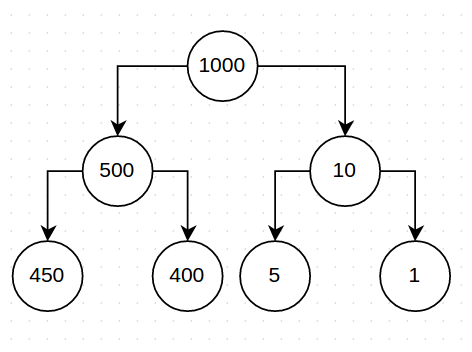
\includegraphics[scale=0.5]{tree.png}
\end{figure} 

Le parcours préfixe de ce tas donne: [1000,500,450,400,10,5,1].

 
\paragraph*{Question 2 (Baptiste Degryse)}
L'algorithme de Knuth-Morris-Pratt, contrairement à l'algorithme de Boyer-Moore, a une sorte de mémoire qui va lui permettre d'identifier les caractères posant régulièrement problème, et de s'adapter afin de limiter le nombre de comparaisons. Il va éviter de refaire x fois la même erreur en comparant des lettres sans importance.\\

La complexité temporelle de cet algorithme est O(m+n), m et n étant la longueur des chaines de caractères à comparer contre une complexité temporelle O(n*m) dans l'algorithme Brute Force. Cette différence est due à la mémoire de la failure fonction dans  KMP. Cette mémoire permet de ne comparer que les caractères les plus problématiques. Exemple de l'utilisation de cette fonction:\\
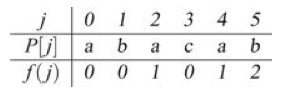
\includegraphics[scale=1]{imgFailure.png}

\paragraph*{Question 3 (Charles Jacquet)} 

Premièrement, on utilise les tries lorsque l'ont a besoin de faire une recherche d'un string dans un texte. Le problème posé est bien le même que pour la question précédente, mais la façon de faire les choses est totalement différente, c'est-à-dire que pour le KMP, on travail sur le string pattern, tandis qu'ici, on travail directement sur le texte, ce qui nous permet d'ailleurs, de faire des recherches différentes en analysant une seule fois le texte.
\begin{itemize}
\item {Compressed trie} : c'est un trie sauf que lorsqu'un noeud à un seul enfant, on rassemble le noeud et son enfant pour éviter ce qu'ils appellent les "redondances".
\item {Gain de place} : Il faut sauvegarder moins de noeud, de plus, il stock les string en dehors de l'arbre, ce qui signifie que dans l'arbre, la complexité spaciale d'un élément est en O(1).
\item {Relation entre un Trie et Suffix Tree} : Un suffix tree, est un trie pour lequel tous les strings stocké dans la collection sont suffix d'un String X.
\end{itemize}
\newpage
\paragraph*{Question 4 (Grynczel Wojciech)}
\textbf{L’algorithme de construction d’un code de Huffman utilise une file de priorité. Est-il avantageux qu’il s’agisse d’une file de priorité adaptable ? Pourquoi ?}

Pas vraiment, la fille de priorité adaptable fournit 3 méthodes en plus :
\begin{itemize}
	\item Entry remove(Entry e);
	\item Object replaceKey(Entry e, Object k);
	\item Object replaceValue(Entry e, Object x);
\end{itemize}

Aucune de ses méthodes ne sera pas utilisée dans l'algorithme de huffman, on supprime toujours les valeurs avec la méthode removeMin(); 

L\textbf{’utilisation d’une file de priorité est-elle indispensable pour pouvoir construire un code de Huffman ? Pouvez-vous imaginer une autre solution en utilisant un algorithme de tri ? }

C’est possible de construire un code de Huffman sans la fille de priorité. Par exemple avec une ArrayList qui sera triée après chaque opération d’insertion.

\textbf{Sa complexité calculatoire serait-elle meilleure que l’algorithme original ? Pourquoi ?}\\
La complexité calculatoire ne sera pas meilleure. Si on utilise une ArrayList on sera obligé de retrier la liste après chaque insert(K key, V velue) afin garder les éléments dans le bon ordre.  


\paragraph*{Question 5 (Ivan)}
Il y a trois étapes dans l’algorithme du Huffman Coding : 
\begin{itemize}


\item L’algorithme calcule d’abord la fréquence de chaque caractère se trouvant dans un string X, et initialise une Priority Queue permettant de stocker les valeurs nécessaires pour créer le coding. 
\item Pour chaque caractère distinct se trouvant dans le string X, l’algorithme crée un arbre binaire T avec un seul noeud, contenant le caractère en question. Ensuite, l’algorithme insert T dans la priority Queue, à la clé qui est égale à la fréquence de ce caractère dans le string X. 
\item Enfin, la boucle while de l’algorithme prend les deux arbres binaires possédant les plus petites fréquences et les fusionne, et ce jusqu’à qu’il ne reste plus qu’un arbre binaire dans la Priority Queue. Chaque itération de cette étape se fait en O(log d) comme complexité temporelle, où d représente le nombre de caractères distincts dans le string X, et ce à l’aide d’une Priority Queue représentée par un Heap. En sachant que cette opération prend deux arbres pour n’en retourner qu’un, et en sachant que cette opération est répétée autant de fois qu’il y a de caractères distincts dans le String X moins une fois, on en déduit que cet algorithme a une complexité temporelle de O(n+d*log d) où d représente le nombre de caractères distincts. 
\end{itemize}


\paragraph*{Question 6 (Bertaux Jérôme)}
Un algorithme de décompression d'un code de Huffman peut se décrire en deux étapes formant une fonction récursive. A chaque itération :
\begin{itemize}
\item Soit le noeud de l'arbre n'est pas une feuille donc on rappel la fonction avec le prochain bit et le fils de gauche si le bit actuel est 0 ou le fils de droite si le bit actuel est 1.
\item Soit le noeud de l'arbre est une feuille, on note alors l'élément se trouvant dans celle-ci. Et on rappel la fonction avec le bit suivant et la racine de l'arbre.
\end{itemize} 
La complexité calculatoire dépend du nombre de bits (n) et est donc de O(n). Pour effectuer l'algorithme nous avons besoin de l'arbre de priorité, d'un texte codé sur forme d'une liste de bit.

\end{document}